\documentclass[12pt,a4paper]{article}
\usepackage{mathptmx} % added for time new roman font
\usepackage[left=0.5in,right=0.5in,top=1in,bottom=1in]{geometry}
\usepackage[latin1]{inputenc}
\usepackage{amsmath}
\usepackage{amsfonts}
\usepackage{amssymb}
\usepackage{graphicx}
\usepackage{float}
\usepackage{booktabs}
\usepackage{parskip} % remove all the paragraph indents


\usepackage{setspace}
\usepackage[colorlinks=true]{hyperref}
\usepackage{textcomp} 
\usepackage{multicol} 

\usepackage{mathtools}          %loads amsmath as well added for the piece wise function
\DeclarePairedDelimiter\Floor\lfloor\rfloor
\DeclarePairedDelimiter\Ceil\lceil\rceil

 
\newcounter{NumberInTable}
\newcommand{\LTNUM}{\stepcounter{NumberInTable}{(\theNumberInTable)}}

\newcommand{\Laplace}[1]{\ensuremath{\mathcal{L}{\left[#1\right]}}}
\newcommand{\InvLap}[1]{\ensuremath{\mathcal{L}^{-1}{\left[#1\right]}}}
\renewcommand{\textuparrow}{$\uparrow$}

\begin{document}
	
	\large{}
	\title{\vspace{-2cm}Lecture Notes, Topic-7}
	\date{}
	\maketitle
	
	\section*{Review from previous class}
	\begin{enumerate}
		\item Harmonic excitations of undamped systems
		\item Harmonic resonance
	\end{enumerate}
	
	\section*{Objectives for today's class}
	\begin{enumerate}
		\item Harmonic excitations of underdamped systems
		\item Frequency response
	\end{enumerate}
	
	\section*{Lecture}
	
		\subsection*{Harmonic excitations of underdamped systems}

			Consider the system
			\begin{figure}[H]
				\centering
				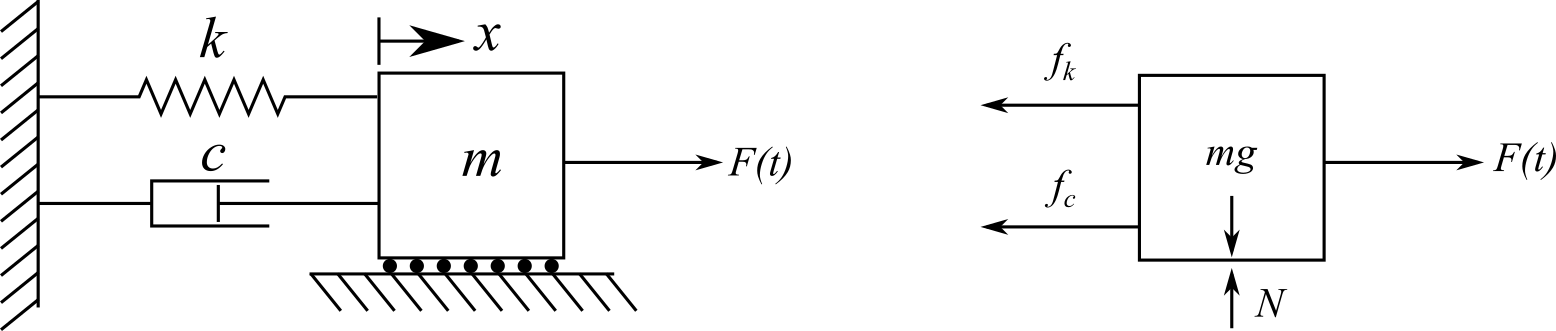
\includegraphics[width=0.7\textwidth]{../../Figures/system_and_FBD_1DOF_damped_forced_horiziontal.png}
			\end{figure}	
			Again, for simplicity let us consider a harmonic excitation for $F(t)$ such that:
			\begin{equation}
				F(t) = F_0\text{cos}(\omega t)
			\end{equation}							
			Summing the forces in the above figure in the $x$ direction yields:
			\begin{equation}
				m \ddot{x}(t)+c\dot{x}(t)+kx(t) = F_0\text{cos}(\omega t)
			\end{equation}			
			For convinces we can convert this to the standard form:					
			\begin{equation}
				\ddot{x}(t)+2 \zeta \omega_n \dot{x}(t) +\omega_n^2x(t) = f_0\text{cos}(\omega t)
			\end{equation}					
			again, where:
			\begin{equation}
				f_0 = \frac{F_0}{m}
			\end{equation}	
			Recall that one way to solve such an equation is to obtain the sum of the homogeneous and particular solutions. 
			\begin{equation}
				x(t) = x_h(t) + x_p(t)
			\end{equation}	
			However, now that we have damping force to consider, out partial solution will have to consider this damping. Therefore:
			\begin{equation}
				x_p(t) = X \text{cos}(\omega t - \phi_p)
			\end{equation}
			where $\phi_p$ represents the phase shift. Note: $\phi_p$ is represented in other texts as $\theta$, $\theta_p$, or even just $\phi$ but we will use $\phi_p$ throughout the remainder of this course. Again, the phase shift is expected because of the effect of the damping force. Now, our total equation is:
			\begin{equation}
				x(t) = Ae^{-\zeta \omega_n t}\text{sin}(\omega_d t + \phi) +  X \text{cos}(\omega t - \phi_p)
			\end{equation}			
			We can use the method of undetermined coefficients to obtain $X$ and $\phi_p$ for the partial solution. First, considering that we write the partial solution in equivalent form:
			\begin{equation}
				x_p(t) = X \text{cos}(\omega t - \phi_p) = A_s \text{cos}(\omega t) + B_s  \text{sin}(\omega t)
			\end{equation}			 
			Taking the derivative of the assumed forms of the partial solution yields:
			\begin{equation}
				x_p(t) = A_s \text{cos}(\omega t) + B_s  \text{sin}(\omega t)
			\end{equation}	
			\begin{equation}
				\dot{x}_p(t) = -\omega A_s \text{sin}(\omega t) + \omega B_s  \text{cos}(\omega t)
			\end{equation}				 
			\begin{equation}
				\ddot{x}_p(t) = -\omega^2 A_s \text{cos}(\omega t) - \omega^2 B_s  \text{sin}(\omega t)
			\end{equation}				
			Recall that the homogeneous and partial solutions are each solution on their own, therefor the EOM can be used to describe just the partial solution. Substituting $x_p$. $\dot{x}_p$, and $\ddot{x}_p$ for $x$. $\dot{x}$, and $\ddot{x}$ in the EOM in standard form $\ddot{x}(t)+2 \zeta \omega_n \dot{x}(t) +\omega_n^2x(t) = f_0\text{cos}(\omega t)$ yields:
			\begin{equation}
			 	\big(	-\omega^2 A_s \text{cos}(\omega t) - \omega^2 B_s  \text{sin}(\omega t) \big)(t)+2 \zeta \omega_n  \big( -\omega A_s \text{sin}(\omega t) + \omega B_s  \text{cos}(\omega t)  \big) (t) +
			\end{equation}
			\begin{equation*}
				\omega_n^2 \big( A_s \text{cos}(\omega t) + B_s  \text{sin}(\omega t) \big)(t) = f_0\text{cos}(\omega t)
			\end{equation*}				
			and rearranging in terms of sin($\omega t$) and cos($\omega t$) yields: 
			\begin{equation}
				(-\omega^2 A_s + 2 \zeta \omega_n \omega B_s + \omega_n^2 A_s -f_0) \text{cos}(\omega t) + 
			\end{equation}
			\begin{equation*}
				(-\omega^2 B_s - 2 \zeta \omega_n \omega A_s + \omega_n^2 B_s)\text{sin}(\omega t) =0
			\end{equation*}	
			considering the two special moments in time $t=(\pi/2)\omega$ and $t=0$ where cos($\omega t$) and sin($\omega t$) equal zero, respectively. Considering $t=(\pi/2)\omega$ results in cos($\omega t$)=0, sin($\omega t$)=1 and the equation simplifies to:
			\begin{equation}
				(-2\zeta \omega_n \omega)A_s + (\omega_n^2 - \omega^2)B_s = 0
			\end{equation}	
			Additionally, at $t=0$, sin($\omega t$)=0 and cos($\omega t$)=1. Therefore, the equation yields		
			\begin{equation}
				(\omega_n^2 - \omega^2)A_s + (2\zeta \omega_n \omega)B_s = f_0
			\end{equation}				
			We can solve two equations for two unknowns. Writing the two linear equations as the singular matrix equation yields:
			\begin{gather}
			   \begin{bmatrix}
			   \omega_n^2 - \omega^2 & 2\zeta \omega_n \omega \\
			   - 2\zeta \omega_n \omega &  \omega_n^2 - \omega^2
			   \end{bmatrix}
  			   \begin{bmatrix}
  			   A_s \\
  			   B_s
  			   \end{bmatrix}
			 = \begin{bmatrix} f_0 \\ 0
			 \end{bmatrix}
			\end{gather}
			This can be solved by computeing the complex inversing, to give us:
			\begin{equation}
				A_s = \frac{(\omega_n^2 - \omega^2)f_0}{(\omega_n^2 - \omega^2)^2 +  (2\zeta \omega_n \omega)^2}
			\end{equation}	
			\begin{equation}
				B_s = \frac{2\zeta \omega_n \omega f_0}{(\omega_n^2 - \omega^2)^2 +  (2\zeta \omega_n \omega)^2}
			\end{equation}	
			From out trigonometric relationships, 
			\begin{equation}
				X = \sqrt{A_s^2 + B_s^2}
			\end{equation}	
			\begin{equation}
				\phi_p = \text{tan}^-1\bigg(\frac{B_s}{A_s}\bigg)
			\end{equation}	
			We can now derive values for our partial solution $x_p$:
			\begin{equation}
				X = \frac{f_0}{\sqrt{(\omega_n^2 - \omega^2)^2 +  (2\zeta \omega_n \omega)^2}} 
			\end{equation}	
			\begin{equation}
				\phi_p = \text{tan}^-1\bigg(\frac{2\zeta \omega_n \omega}{\omega_n^2 - \omega^2}\bigg)
			\end{equation}				
			Now we can build a solution for the partial equation ($x_p$), therefore, the total solution becomes:
			\begin{equation}
				x(t) = x_h(t) + x_p(t)
			\end{equation}
			\begin{equation}
				x(t) = Ae^{-\zeta \omega_n t}\text{sin}(\omega_d t + \phi) +  X \text{cos}(\omega t - \phi_p)
			\end{equation}				
			Note for larger values of $t$, the homogeneous solution approaches zero resulting in the partial solution becoming the total solution. Therefore, the partial solution is sometimes called the \textbf{steady state response} and the homogeneous solution is called the \textbf{transient response}. Solving for the constants $A$ and $\phi$ using boundary conditions ($x_0=0$ and $v_0=0$) results a total solution expressed as:
			\begin{equation}
				A = \frac{x_0 -X \text{cos}(\phi_p)}{\text{sin}(\phi)}
			\end{equation}			 
			\begin{equation}
				\phi =  \text{tan}^-1\bigg(\frac{\omega_d ( x_0 -X \text{cos}(\phi_p))}{v_0 + (x_0 - X \text{cos}(\phi_p)) \zeta \omega_n - \omega X \text{sin}(\phi_p) }\bigg)
			\end{equation}			
			Finally, assembling all the terms:
			\begin{equation}
				x(t) = Ae^{-\zeta \omega_n t}\text{sin}(\omega_d t + \phi) +  X \text{cos}(\omega t - \phi_p)
			\end{equation}
			\begin{equation}
				A = \frac{x_0 -X \text{cos}(\phi_p)}{\text{sin}(\phi)}
			\end{equation}			 
			\begin{equation}
				\phi =  \text{tan}^-1\bigg(\frac{\omega_d ( x_0 -X \text{cos}(\phi_p))}{v_0 + (x_0 - X \text{cos}(\phi_p)) \zeta \omega_n - \omega X \text{sin}(\phi_p) }\bigg)
			\end{equation}	
			\begin{equation}
				X = \frac{f_0}{\sqrt{(\omega_n^2 - \omega^2)^2 +  (2\zeta \omega_n \omega)^2}} 
			\end{equation}	
			\begin{equation}
				\phi_p = \text{tan}^-1\bigg(\frac{2\zeta \omega_n \omega}{\omega_n^2 - \omega^2}\bigg)
			\end{equation}							
			Let's consider how these equation play out in a real system. Again, consider the system
			\begin{figure}[H]
				\centering
				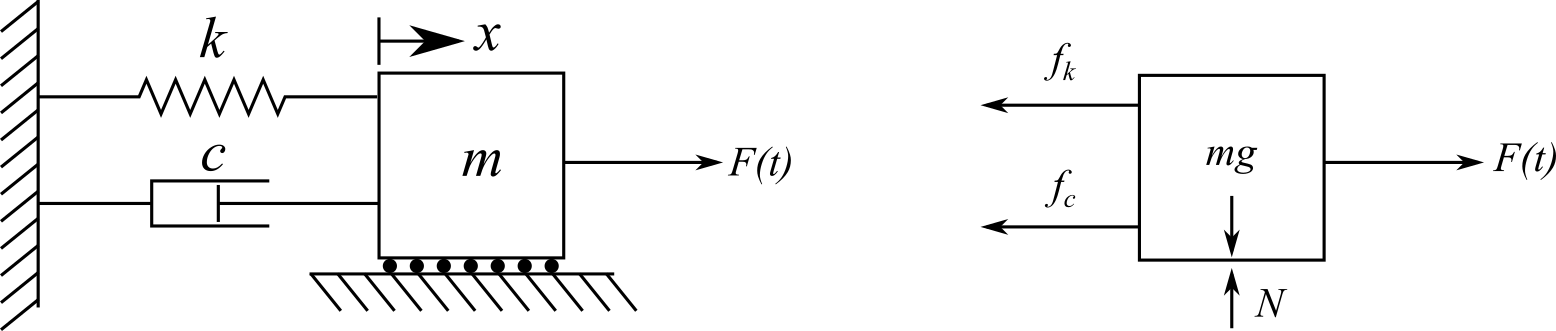
\includegraphics[width=0.7\textwidth]{../../Figures/system_and_FBD_1DOF_damped_forced_horiziontal.png}
			\end{figure}			
			If we plot the total, transient, and steady state responses for $k=100$ N/m, $m=10$ kg,  $c=10$ kg/s, $F_0=1$ N, $\omega=3.162$ rad/sec, and no initial conditions we get:
			\begin{figure}[H]
				\centering
				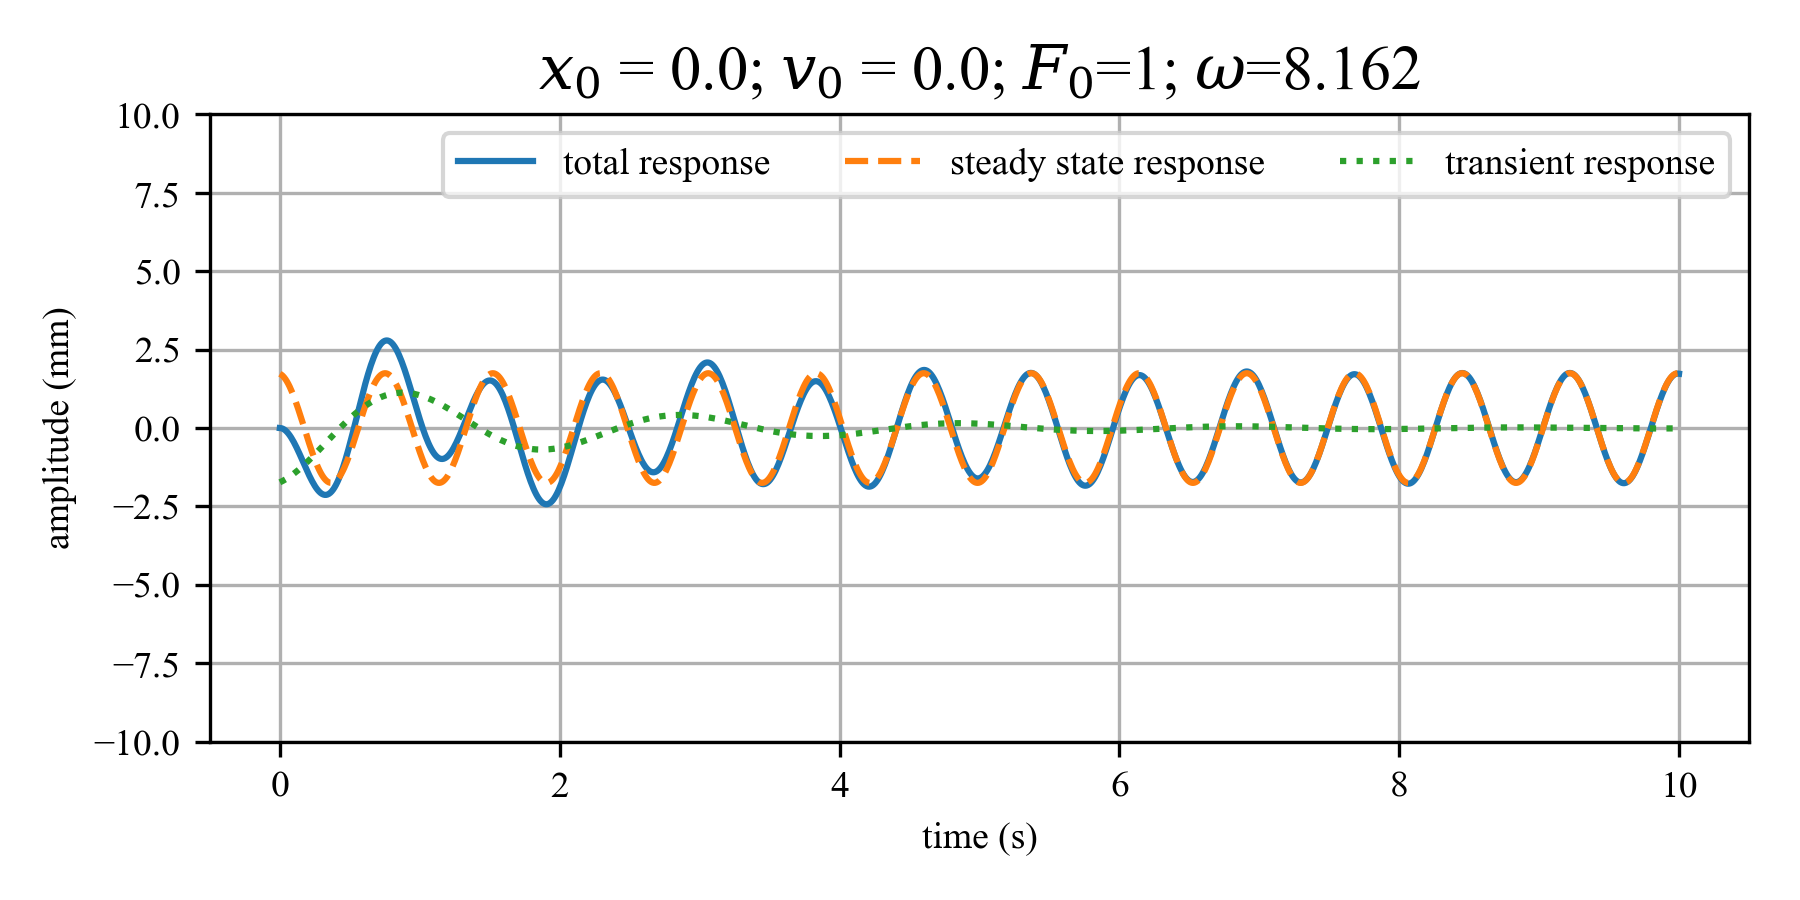
\includegraphics[width=0.7\textwidth]{../../Figures/example_1_1.png}
			\end{figure}			
			If we increase the forcing function $F_0$ to 3 N we get:
			\begin{figure}[H]
				\centering
				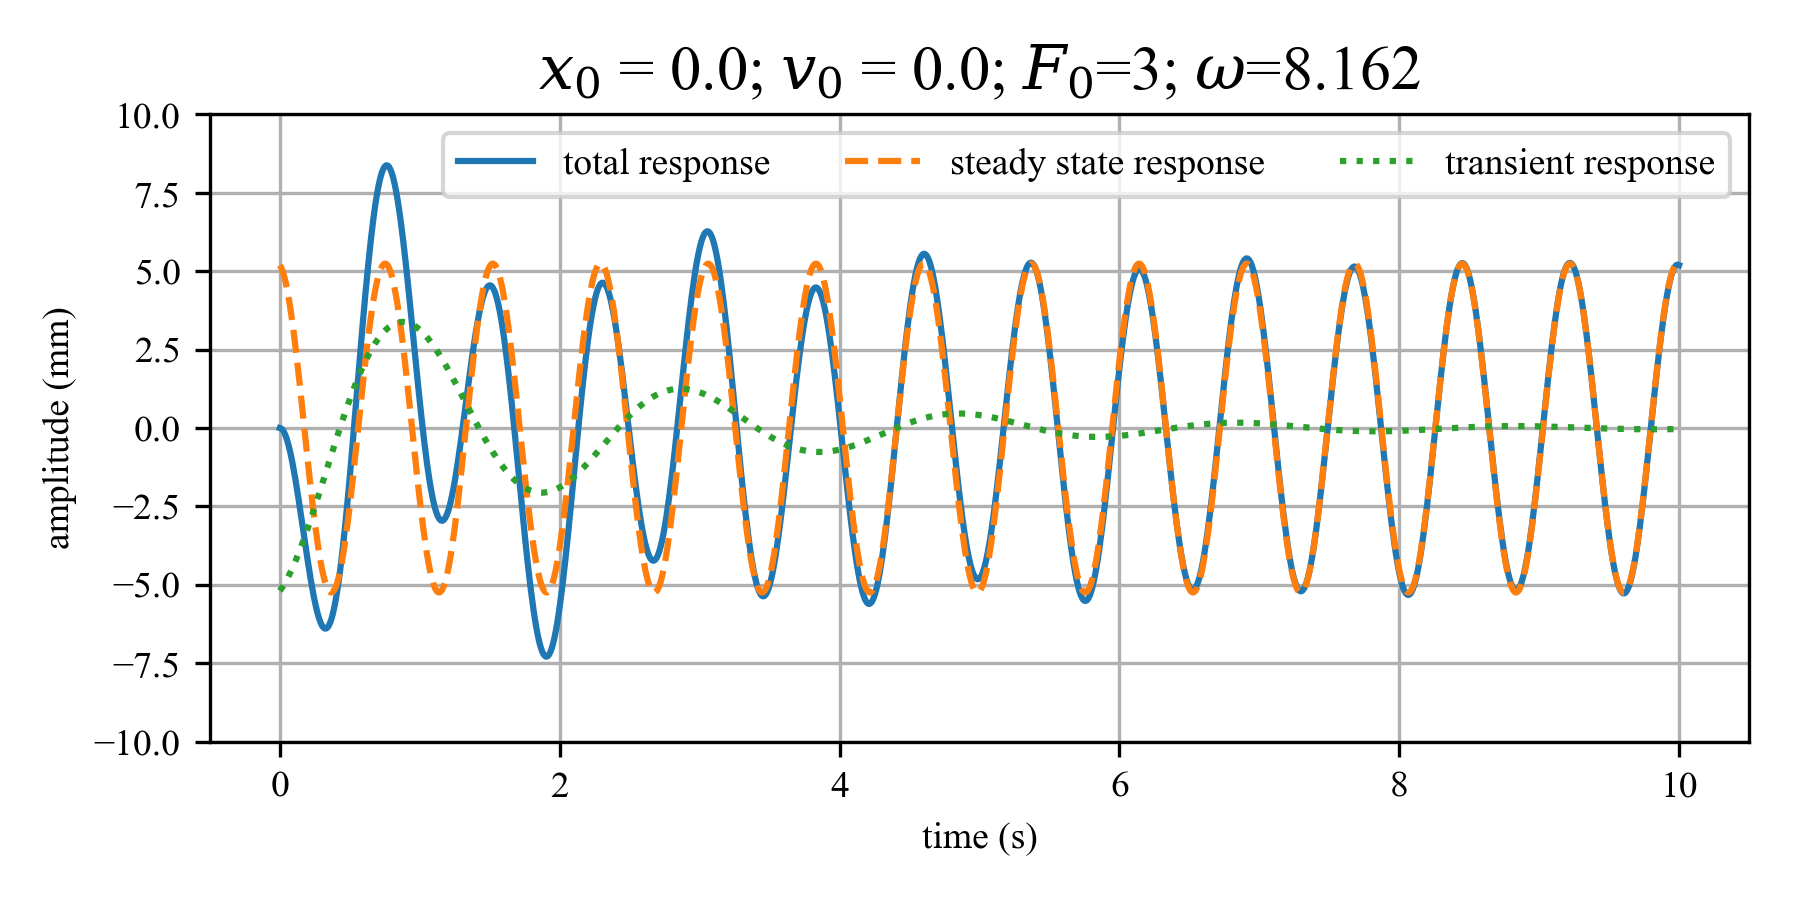
\includegraphics[width=0.7\textwidth]{../../Figures/example_1_2.png}
			\end{figure}			
			now, using $F_0=1$ N, but setting $\omega=5$ rad/sec we get:
			\begin{figure}[H]
				\centering
				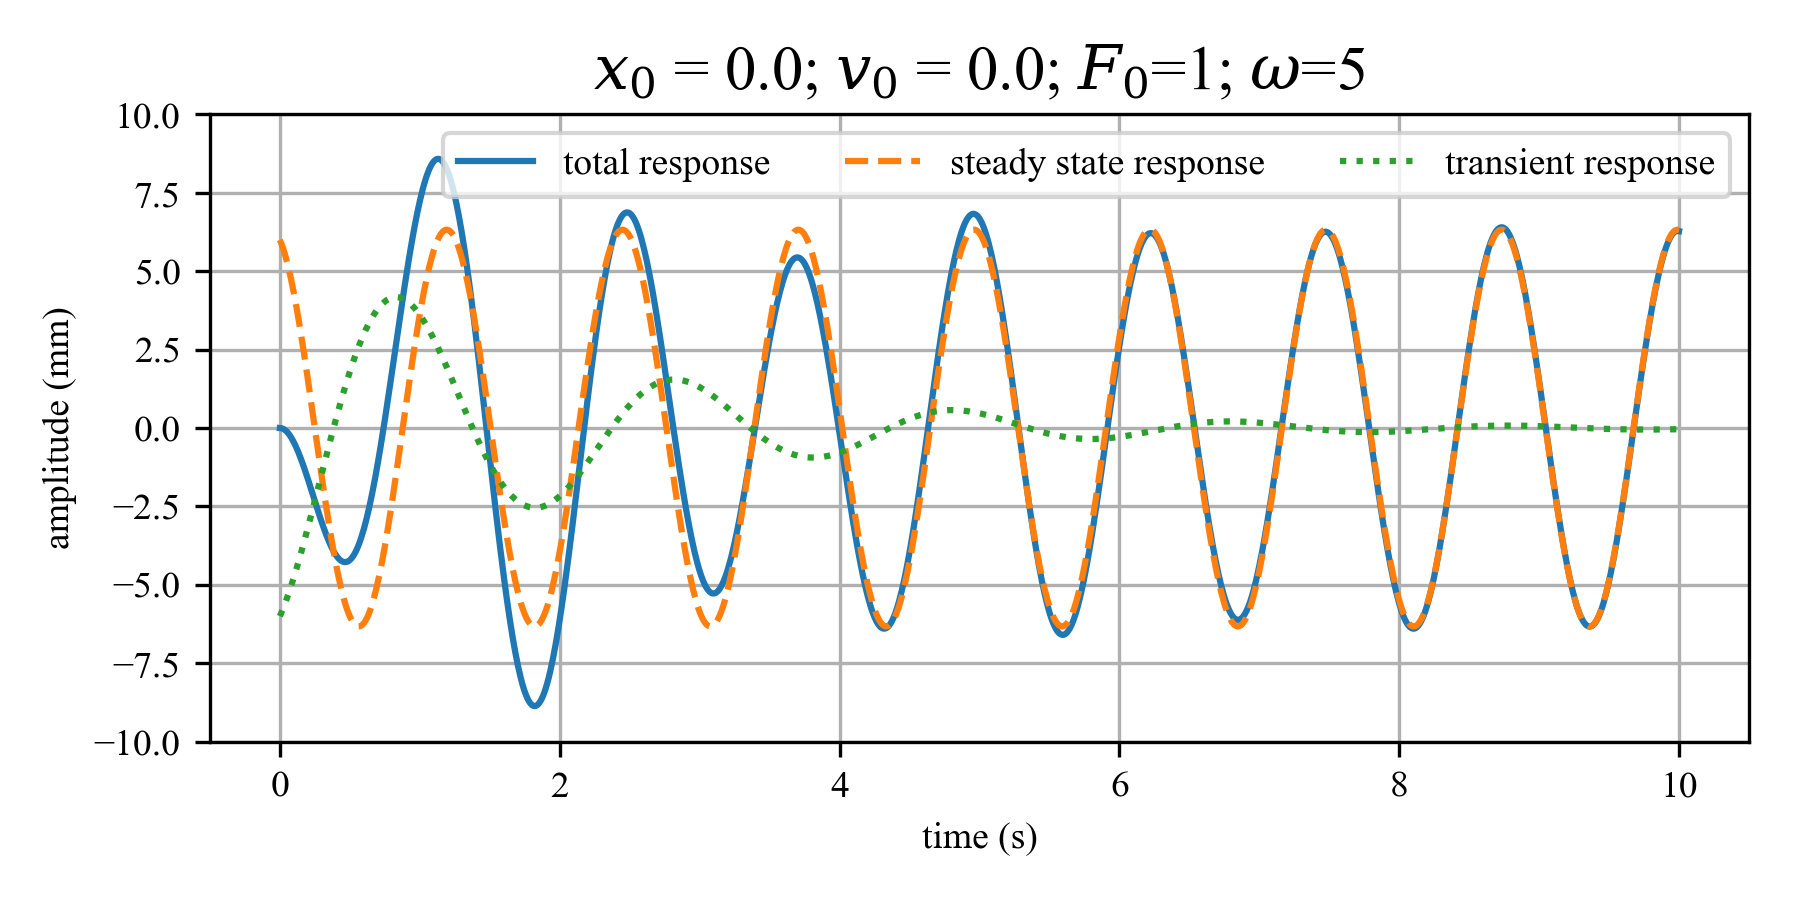
\includegraphics[width=0.7\textwidth]{../../Figures/example_1_3.png}
			\end{figure}				
			This is because $\omega$ is closer to the natural frequency $\omega_n$. Setting $\omega=\omega_n$ we get
			\begin{figure}[H]
				\centering
				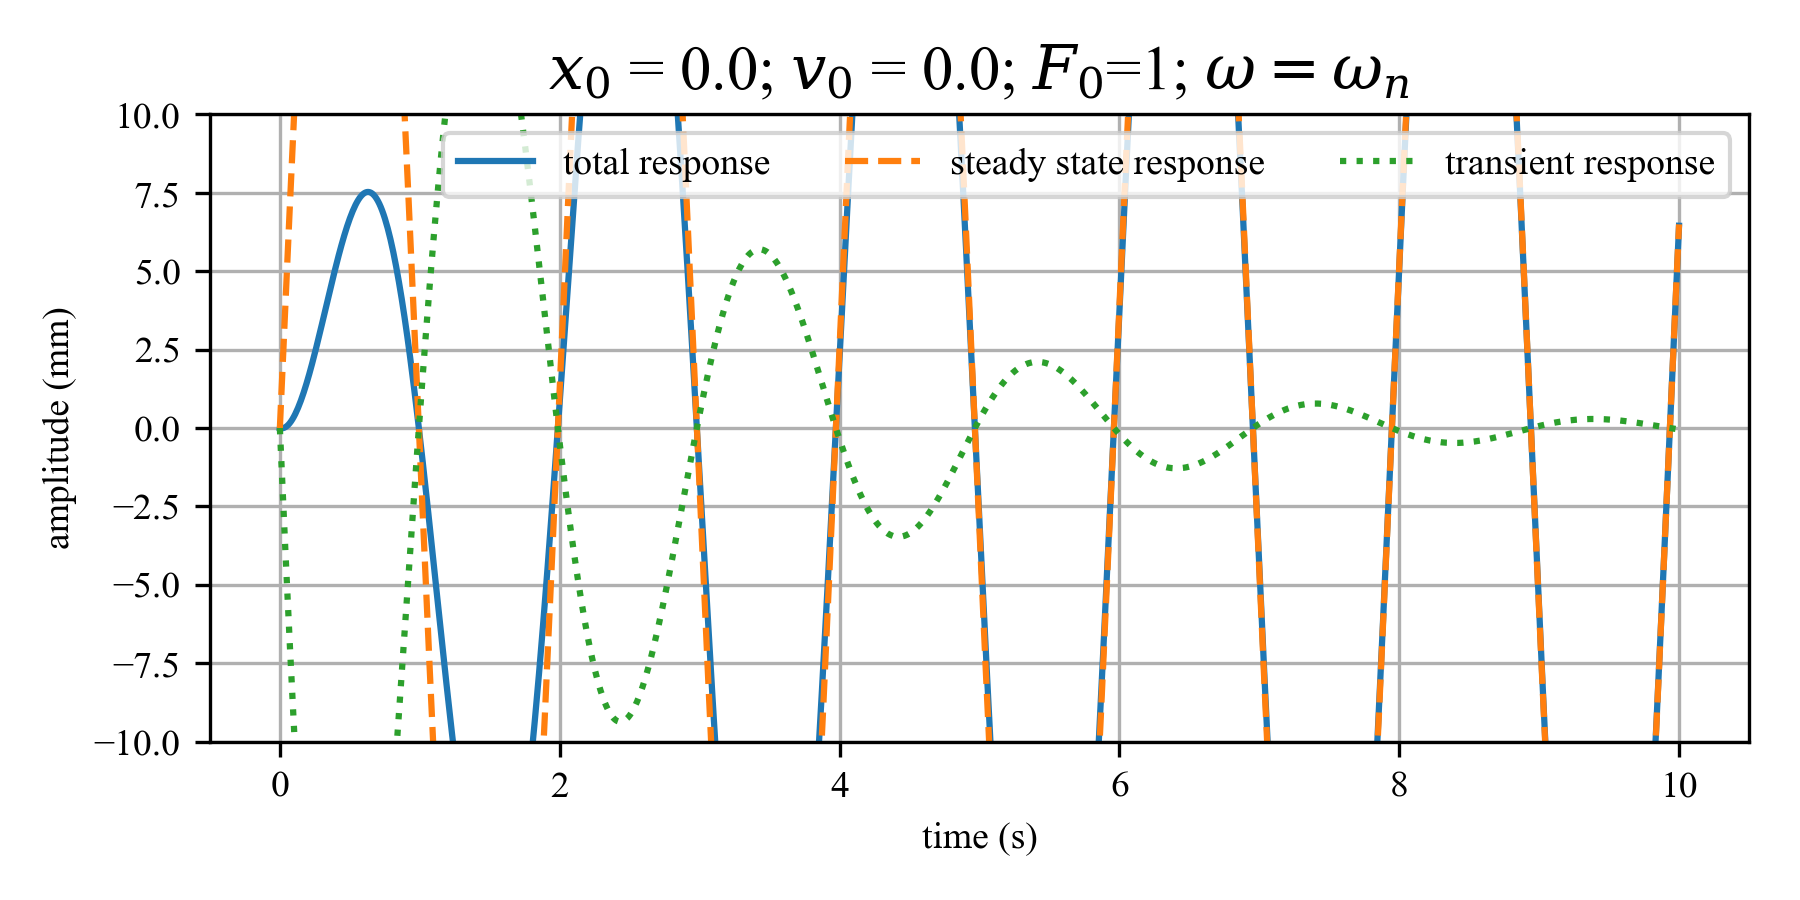
\includegraphics[width=0.7\textwidth]{../../Figures/example_1_4.png}
			\end{figure}			
			As expected, setting $\omega=\omega_n$ causes the system to enter into resonance. However, this is different than resonance for a undamped system in that the amplitude of the displacement is not unbounded (recall that the damper will absorb energy). So if we scale the plot correctly we get: 
			\begin{figure}[H]
				\centering
				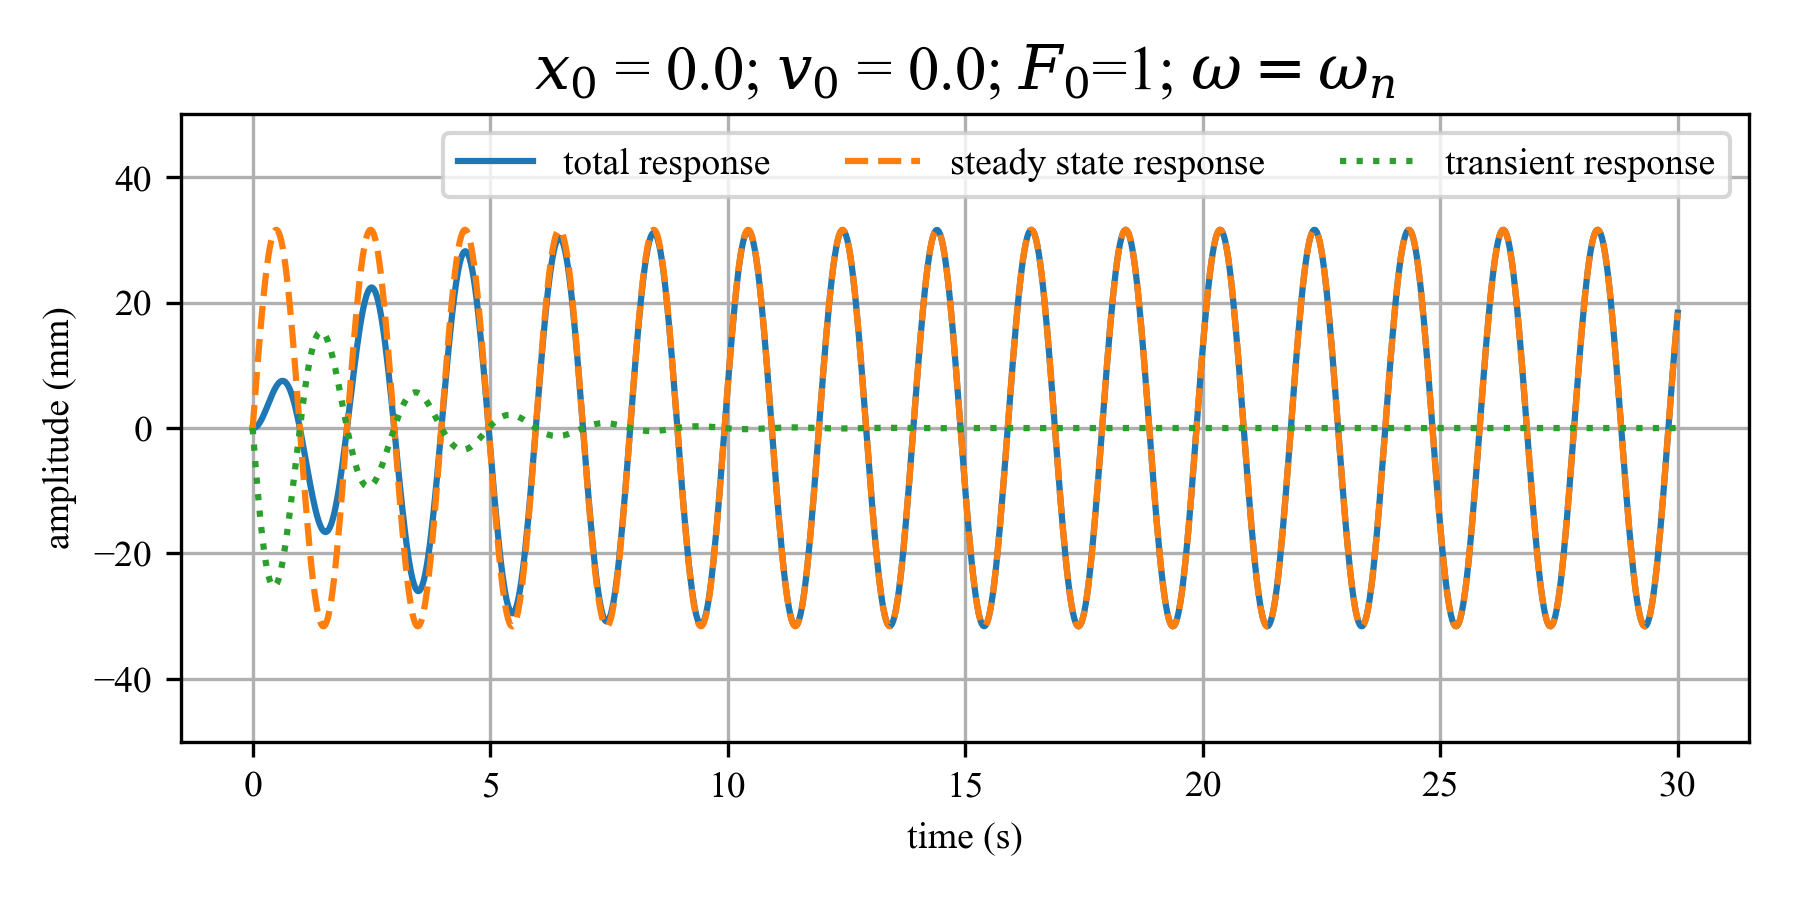
\includegraphics[width=0.7\textwidth]{../../Figures/example_1_5.png}
			\end{figure}
			
			From the figure we can see that for larger values of $t$ the transient response dies out while only the steady state response controls the displacement of the total response. This is always true if the system has any significant damping. Therefore, it is often prudent to ignore the transient part and focus only on the steady-state response. Considering the equation for the partial solution: 
			\begin{equation}
				x_p(t) = X \text{cos}(\omega t - \phi_p)
			\end{equation}			 
			and knowing the values for $X$ and $\phi_p$: 
			\begin{equation}
				X = \frac{f_0}{\sqrt{(\omega_n^2 - \omega^2)^2 +  (2\zeta \omega_n \omega)^2}} 
			\end{equation}	
			\begin{equation}
				\phi_p = \text{tan}^-1\bigg(\frac{2\zeta \omega_n \omega}{\omega_n^2 - \omega^2}\bigg)
			\end{equation}	
			We want to find a way to plot the responses of the system only in terms of terms of the system's natural and driving frequencies, and its damping. First, we define a frequency ratio as the dimensionless quantity 
			\begin{equation}
				r = \frac{\omega}{\omega_n}
			\end{equation}
			\textbf{Another common way to express $r$ is $\beta$}. Next, Recall that:
			\begin{equation}
				X = \frac{f_0}{\sqrt{(\omega_n^2 - \omega^2)^2 +  (2\zeta \omega_n \omega)^2}}  = \frac{\frac{F_0}{m}}{\sqrt{(\omega_n^2 - \omega^2)^2 +  (2\zeta \omega_n \omega)^2}} 
			\end{equation}				
			If we factor out $\omega_n^2$ from the denominator and substitute in $\omega_n^2 = k/m$ and $r = \omega/\omega_n$, we get:
			\begin{equation}
				X = \frac{\frac{F_0}{m}}{\omega_n^2 \sqrt{\big(1 - (\frac{\omega}{\omega_n})^2\big)^2 +  (2\zeta \frac{\omega}{\omega_n})^2}} =  \frac{\frac{F_0}{k}}{\sqrt{(1-r^2)^2+(2\zeta r)^2}}
			\end{equation}				
			this becomes:
			\begin{equation}
				\frac{Xk}{F_0} = \frac{X \omega_n^2}{f_0} = \frac{1}{\sqrt{(1-r^2)^2+(2\zeta r)^2}}
			\end{equation}				
			in a similar fashion, if we manipulate the equation for $\phi_p$ we can get $\phi_p$ in term of $r$:
			\begin{equation}
				\phi_p = \text{tan}^-1\bigg(\frac{2 \zeta r}{1-r^2}\bigg)
			\end{equation}	
			If we solve for a few key values of $r$ we can get the following data points. On the board, we can solve for a few different frequency responses for a few different damping coefficients. 
			\begin{table}[H]
				\centering
				\begin{tabular}{@{}lccccccccc@{}}
				\toprule
				 & & \multicolumn{5}{c}{frequency ration ($r$)} \\ 
				$r$ & 0 & 0.25& 0.5& 0.75& 1& 1.25& 1.5& 1.75& 2.0 \\ \midrule
				$\zeta=0.7$	&	1.00&  1.00	&   0.97&	0.88&	0.71&	0.54&	0.41&	0.31 & 0.24\\
				$\zeta=0.5$	&	1.00&	1.03&	1.11&	1.15&	1.00&	0.73&	0.51&	0.37 & 0.28\\ 
				$\zeta=0.25$	&	1.00&	1.03&	1.11&	1.15&	1.00&	0.73&	0.51&	0.37 & 0.28 \\ 
				$\zeta=0.1$	&	1.00&	1.07&	1.32&	2.16&	5.00&	1.62&	0.78&	0.48 & 0.33 \\ \bottomrule
				\end{tabular}
			\end{table}
			If we plot the values of the normalize amplitude vs $r$ we obtain:
			\begin{figure}[H]
				\centering
				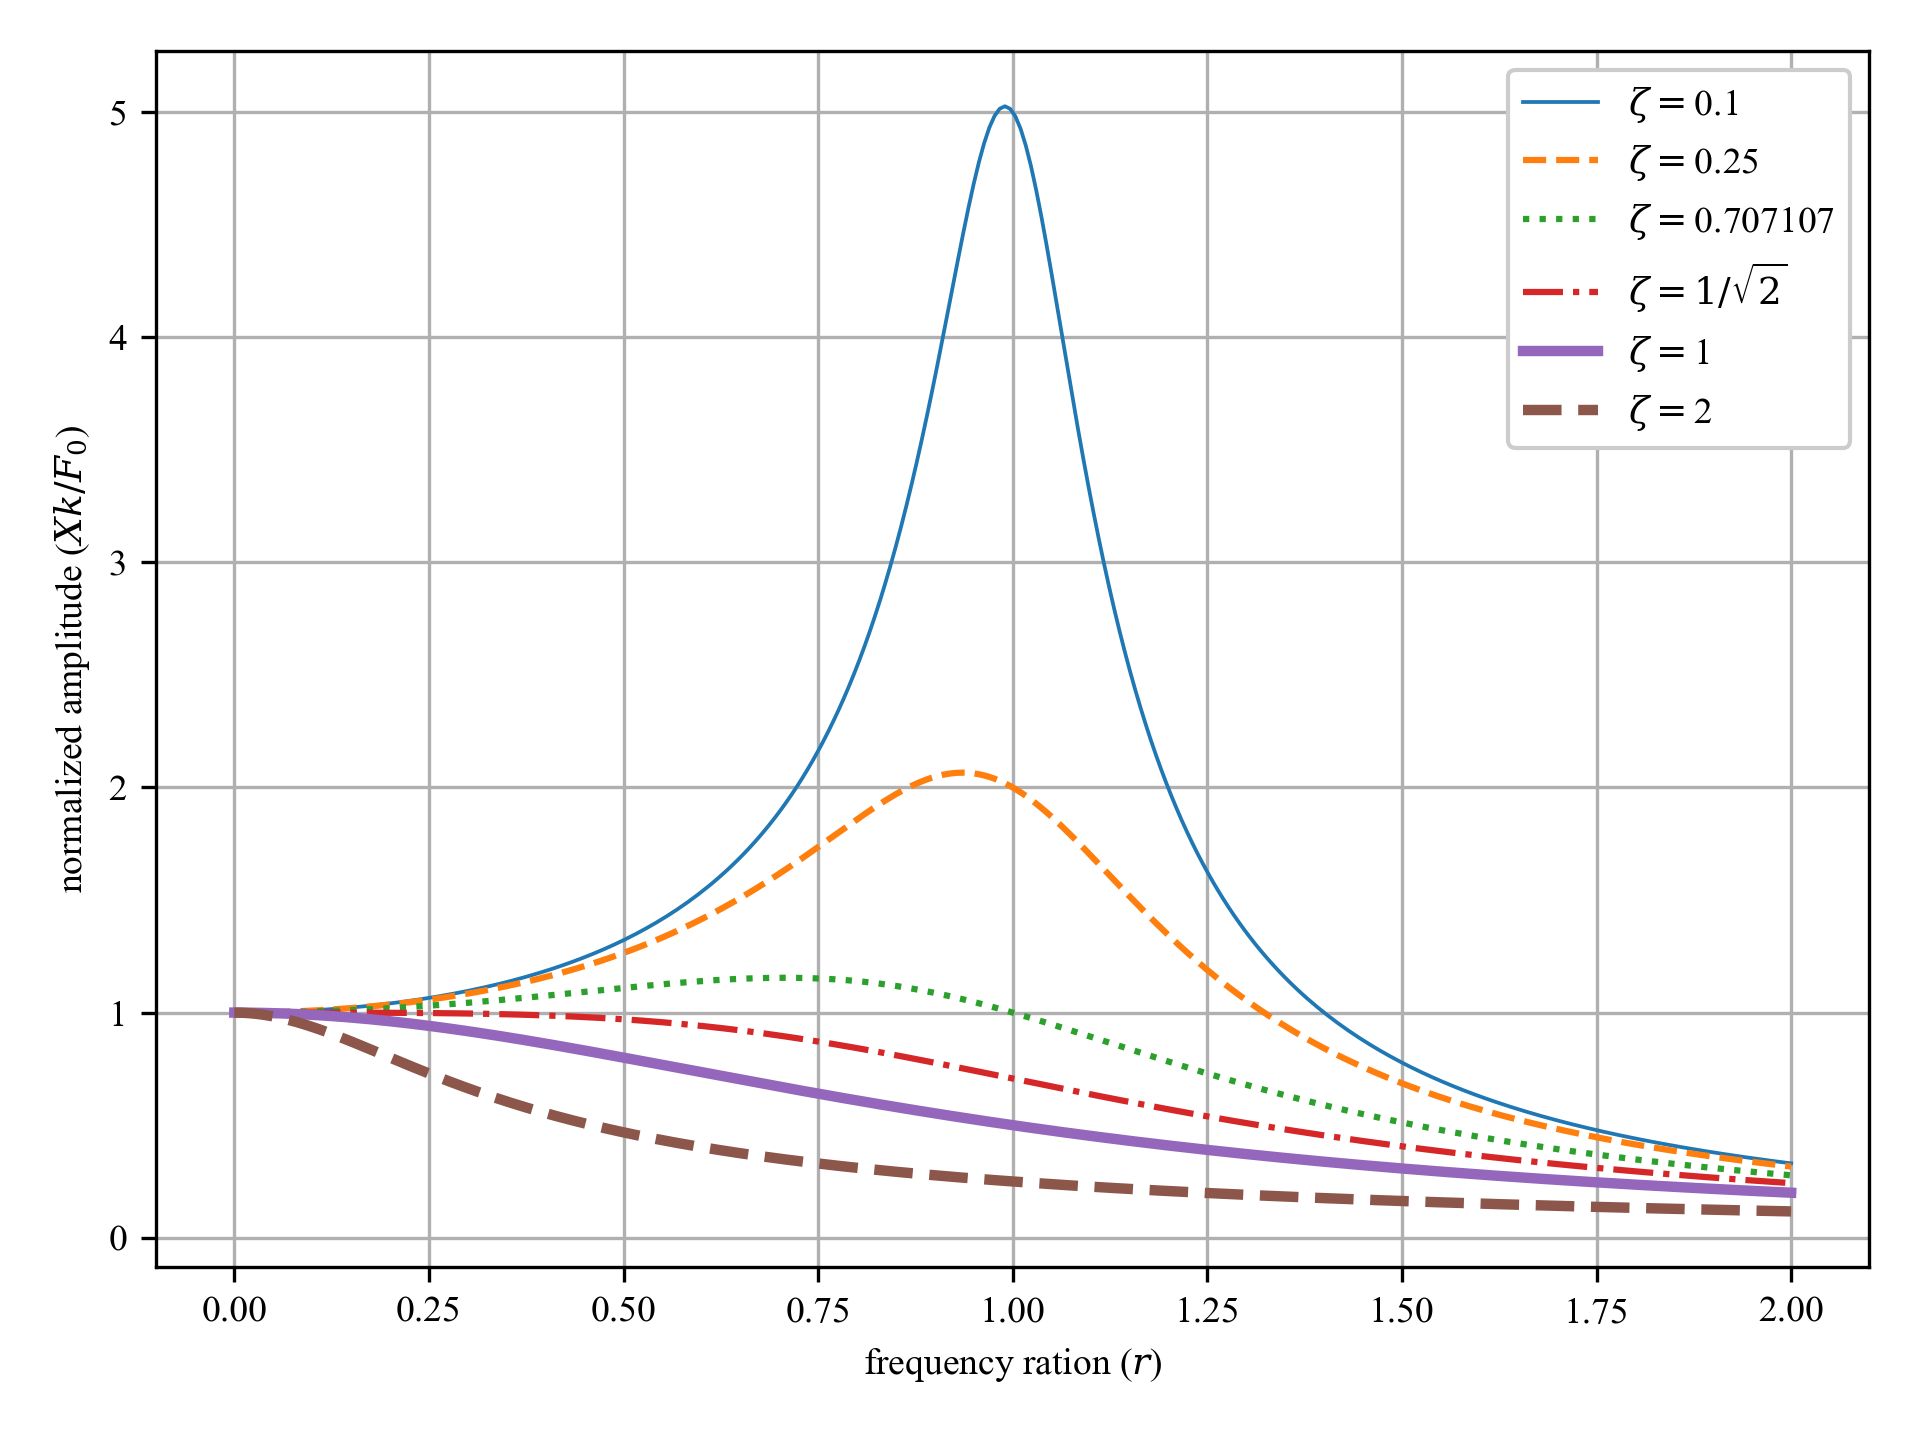
\includegraphics[width=0.8\textwidth]{../../Figures/frequency_response_amplitude.png}
			\end{figure}			
			And again, if we plot the values of the phase vs $r$ ($\omega/\omega_n$) we obtain:
			\begin{figure}[H]
				\centering
				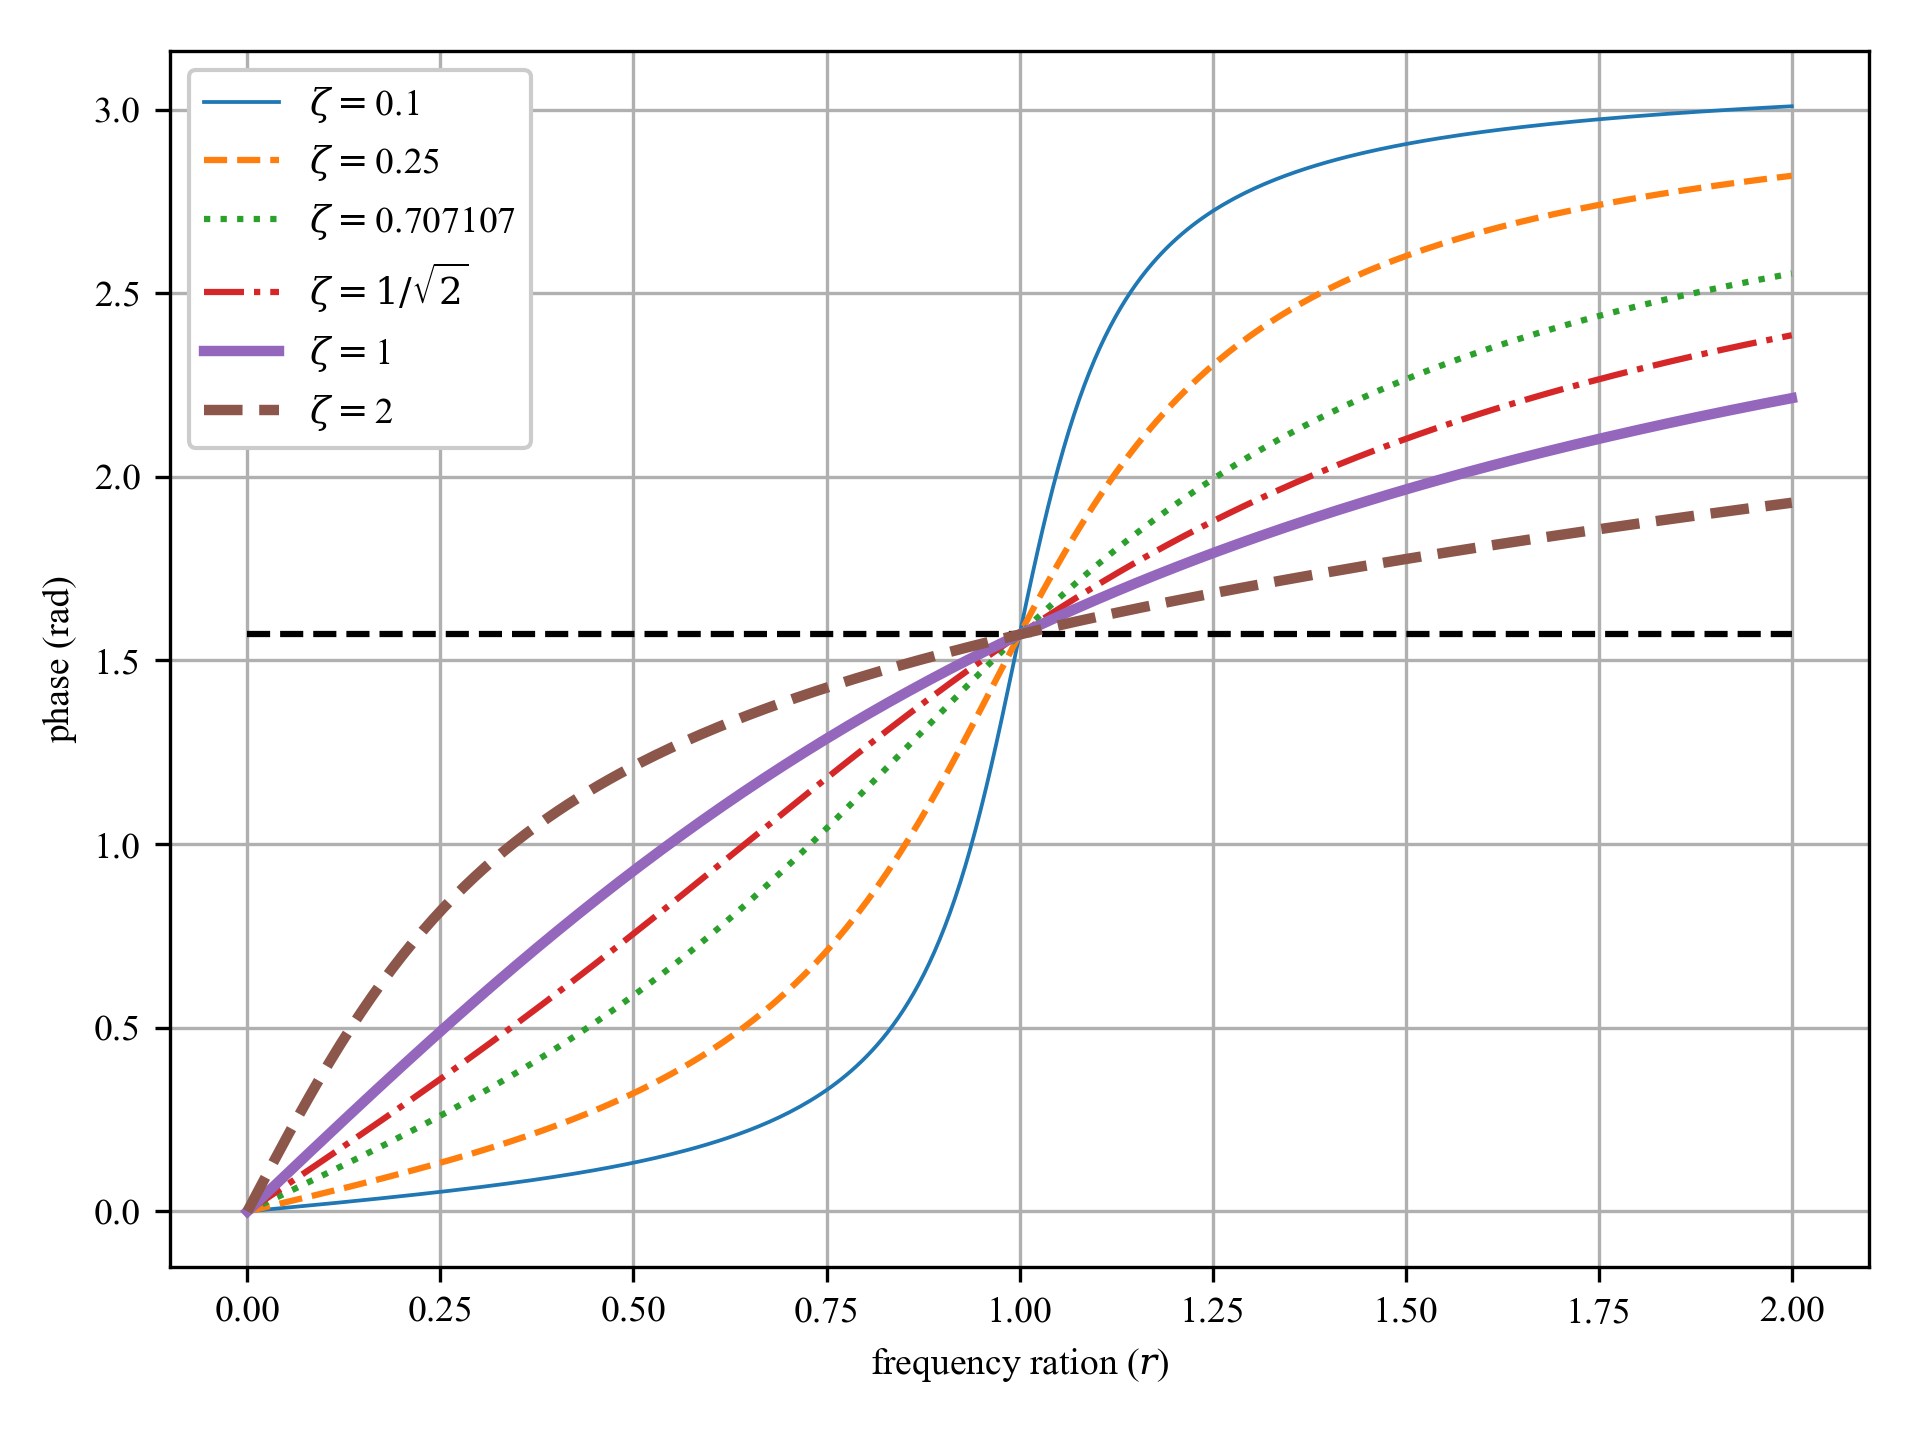
\includegraphics[width=0.8\textwidth]{../../Figures/frequency_response_phase.png}
			\end{figure}				
			note that the dashed black line is there because the phase value after $\pi/2$ need to be adjusted to obtain a continuous plot. An astute observer would notice that the maximum amplitude is not at $\omega = \omega_n$. While resonance is defined as $\omega = \omega_n$, this does not define the point of maximum displacement of the steady state response. Let us solve for the frequency ratio with the maximum displacement. This will happen when
			\begin{equation}
				\frac{d}{dr}\Bigg(\frac{Xk}{F_0} \Bigg)= 0
			\end{equation}				
			We can show that:
			\begin{equation}
			\Bigg(\frac{1}{\sqrt{(1-r^2)^2+(2\zeta r)^2}}\Bigg)	\frac{d}{dr} =0
			\end{equation}	
			when 
			\begin{equation}
			r_{\text{peak}} = \sqrt{1-2 \zeta^2}= \frac{\omega_p}{\omega_n}, \hspace{1cm} \zeta<1/\sqrt{2} 
			\end{equation}				
			however, this is only true for under damped system in which $\zeta<1/\sqrt{2}$. If $\zeta>1/\sqrt{2}$ than the value in imaginary and the peak value is at $r=0$. In these cases, the maximum displacement is a function of only $\omega_n$. $\omega_p$ represents the driving frequency that correspond to the maximum amplitude ($\frac{Xk}{F_0}$) and is called the \textbf{peak frequency}, and can be calculated as:
			\begin{equation}
			\omega_p = \omega_n r_{\text{peak}} = \omega_n \sqrt{1-2 \zeta^2}, \hspace{1cm} \zeta<1/\sqrt{2} 
			\end{equation}				
			
			
			
		\subsection*{Example 1}
			Consider the simple spring mass system, 
			\begin{figure}[H]
				\centering
				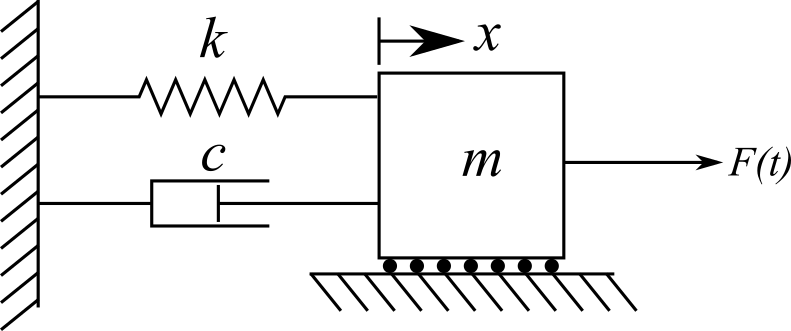
\includegraphics[width=0.4\textwidth]{../../Figures/system_1DOF_horiziontal_damped_forced.png}
			\end{figure}				
			where $\omega_n = 132$ rad/sec and $\zeta$ = 0.0085. Calculate the displacements of the steady-state response for $\omega$=132 and 125 rad/sec. In both cases, use $f_0$ = 10 N/kg. 

			\textbf{Solution}
			
			From before, we know the solution for the displacement of the partial solution for $\omega$=132 rad/sec is:
			\begin{equation}
				X = \frac{f_0}{\sqrt{(\omega_n^2 - \omega^2)^2 +  (2\zeta \omega_n \omega)^2}} = \frac{10}{2(0.0085)(132)^2} = 0.034 \text{ m}
			\end{equation}							
			while for $\omega$=125 rad/sec X is:
			\begin{equation}
				X = \frac{f_0}{\sqrt{(\omega_n^2 - \omega^2)^2 +  (2\zeta \omega_n \omega)^2}} = \frac{10}{\sqrt{(1799)^2 +  (280.5)^2}}  = 0.005 \text{ m}
			\end{equation}				
			Therefore, a slight change in the driving frequency (about 5\%) results in a 85\% change in the amplitude of the steady-state response. 
			
		\subsection*{Example 2}
			The steady state response for an engineered system must not surpass 1 cm, if the system can be modeled as the spring and mass system below, what value of $c$ must be used?  
			\begin{figure}[H]
				\centering
				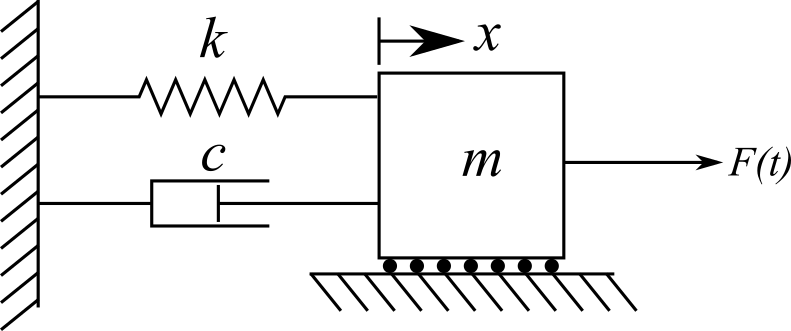
\includegraphics[width=0.4\textwidth]{../../Figures/system_1DOF_horiziontal_damped_forced.png}
			\end{figure}	
			Use $k$ = 2000 N/m, $m$ = 100 kg, $F(t)$ = 20 cos($6.3t$) N. 			

			\textbf{Solution}
			The steady state solution is:
			\begin{equation}
				x_p(t) = X \text{cos}(\omega t - \phi_p)
			\end{equation}			 
			knowing the amplitude is controlled by $X$: 
			\begin{equation}
				X = \frac{f_0}{\sqrt{(\omega_n^2 - \omega^2)^2 +  (2\zeta \omega_n \omega)^2}} 
			\end{equation}	
			and recalling from the EOM in standard form that $2\zeta \omega_n = c/m$ we can obtain:
			\begin{equation}
				X = \frac{f_0}{\sqrt{(\omega_n^2 - \omega^2)^2 +  (\frac{c}{m} \omega)^2}} 
			\end{equation}		
			rearranging for $c$ gives:		
			\begin{equation}
				c = m\sqrt{\frac{f_0^2}{\omega^2 X^2}-\frac{\big(\omega_n^2-\omega^2\big)^2}{\omega^2}} = \sqrt{\frac{F_0^2}{\omega^2 X^2}-m^2\frac{\big(\omega_n^2-\omega^2\big)^2}{\omega^2}} 
			\end{equation}
			Therefore, if we set $X=0.01$ m we can solve the above equation to yield $c$ = 55.7 kg/s.

\end{document}


























